\documentclass{article}

% If you're new to LaTeX, here's some short tutorials:
% https://www.overleaf.com/learn/latex/Learn_LaTeX_in_30_minutes
% https://en.wikibooks.org/wiki/LaTeX/Basics

% Formatting
\usepackage[utf8]{inputenc}
\usepackage[margin=1in]{geometry}
\usepackage[titletoc,title]{appendix}
\usepackage{placeins}
% \usepackage{authblk}
% \usepackage{multirow}

% Math
% https://www.overleaf.com/learn/latex/Mathematical_expressions
% https://en.wikibooks.org/wiki/LaTeX/Mathematics
\usepackage{amsmath,amsfonts,amssymb,mathtools}

% Images
% https://www.overleaf.com/learn/latex/Inserting_Images
% https://en.wikibooks.org/wiki/LaTeX/Floats,_Figures_and_Captions
\usepackage{graphicx,float}
\usepackage{subfig}

% Tables
% https://www.overleaf.com/learn/latex/Tables
% https://en.wikibooks.org/wiki/LaTeX/Tables

% Algorithms
% https://www.overleaf.com/learn/latex/algorithms
% https://en.wikibooks.org/wiki/LaTeX/Algorithms
\usepackage[ruled,vlined]{algorithm2e}
\usepackage{algorithmic}

% Code syntax highlighting
% https://www.overleaf.com/learn/latex/Code_Highlighting_with_minted
\usepackage{minted}
\usemintedstyle{borland}

% References
% https://www.overleaf.com/learn/latex/Bibliography_management_in_LaTeX
% https://en.wikibooks.org/wiki/LaTeX/Bibliography_Management
\usepackage{biblatex}
\addbibresource{references.bib}

% Listings
% https://www.overleaf.com/learn/latex/Code_listing
\usepackage{listings}
\usepackage{xcolor}

% URLs
% https://www.overleaf.com/learn/latex/Hyperlinks
\usepackage{hyperref}
\hypersetup{
    colorlinks=true,
    linkcolor=blue,
    filecolor=magenta,      
    urlcolor=blue,
}
 
\urlstyle{same}
 
\definecolor{codegreen}{rgb}{0,0.6,0}
\definecolor{codegray}{rgb}{0.5,0.5,0.5}
\definecolor{codepurple}{rgb}{0.58,0,0.82}
\definecolor{backcolour}{rgb}{0.95,0.95,0.92}
 
\lstdefinestyle{mystyle}{
    backgroundcolor=\color{backcolour},   
    commentstyle=\color{codegreen},
    keywordstyle=\color{magenta},
    numberstyle=\tiny\color{codegray},
    stringstyle=\color{codepurple},
    basicstyle=\ttfamily\footnotesize,
    breakatwhitespace=false,         
    breaklines=true,                 
    captionpos=b,                    
    keepspaces=true,                 
    numbers=left,                    
    numbersep=5pt,                  
    showspaces=false,                
    showstringspaces=false,
    showtabs=false,                  
    tabsize=2
}
 
\lstset{style=mystyle}

% Title content
\title{AMATH 582 Final: Data Analysis on CLT Rocking Shear Walls}
%\author{Sarah Wichman, Chi-Pu (Tom) Lin, and Nicolette Lewis}
% \author[1]{Sarah Wichman}
% \author[1]{Chi-Pu (Tom) Lin}
% \author[1]{Nicolette Lewis}
% \affil[1]{Ph.D. Candidate, Department of Civil and Environmental Engineering, University of Washington, Seattle}
\author{Sarah Wichman\thanks{Ph.D. Candidate, Department of Civil and Environmental Engineering, University of Washington, Seattle} , Chi-Pu (Tom) Lin\footnotemark[1] , and Nicolette Lewis\footnotemark[1]}
\date{March 19, 2020}

\begin{document}
\maketitle

% Abstract
\begin{abstract}
    Accelerometer data from the NHERI TallWood test on a full-scale two-story shake table test on a timber building was used to study the modal properties of the specimen. Many techniques in data analysis were utilized including Gaussian filters, averaging filters, Fourier transforms, spectrograms and SVDs. Using these techniques, investigations into dynamical information about the specimen that hadn't previously been explored were completed. 
\end{abstract}

\FloatBarrier
% Introduction and Overview
\section{Introduction and Overview}

With the development of engineered wood products such as cross laminated timber (CLT), tall timber buildings are becoming feasible and offer benefits such as faster construction and the use of sustainable building materials. It has also opened the door to creating seismic resilient systems that sustain minor damage during large earthquakes. With this in mind, the NHERI TallWood Project, funded by the National Science Foundation, is developing a rocking CLT wall seismic force resisting system for tall timber buildings. During the summer of 2017, the NHERI TallWood group tested a full-scale two-story mass timber building (Fig.\ \ref{fig:Building}), with CLT post-tensioned rocking walls as the lateral system at the NHERI Large High Performance Outdoor Shake Table at the University of California, San Diego (UCSD).

\medskip

Extensive analysis of the behavior of this specimen has been conducted to study how the building performed and the potential for using timber to create a seismically resilient structure. These previous studies have looked closely at the the overall displacements of the structure and the movements of each individual component to study how susceptible it is to damage \cite{Pei}, \cite{DeMeza}, and \cite{Wichman}. Limited work however has been conducted to study the modal response of this specimen during the test. This report aims to fill those gaps and to look at the overall modal response of the structure by leveraging different data analysis technique (e.g.\ Fourier transform, spectrograms, and singular value decomposition).

\medskip

The data used in this report was obtained by Sarah Wichman (co-author of this report) and the rest of the NHERI TallWood group \cite{TallWood}. All data is publicly available on the NHERI DesignSafe cyberinfrastructre \cite{DesignSafe}.

\begin{figure}[!htbp]
    \centering
    \subfloat[Photo]{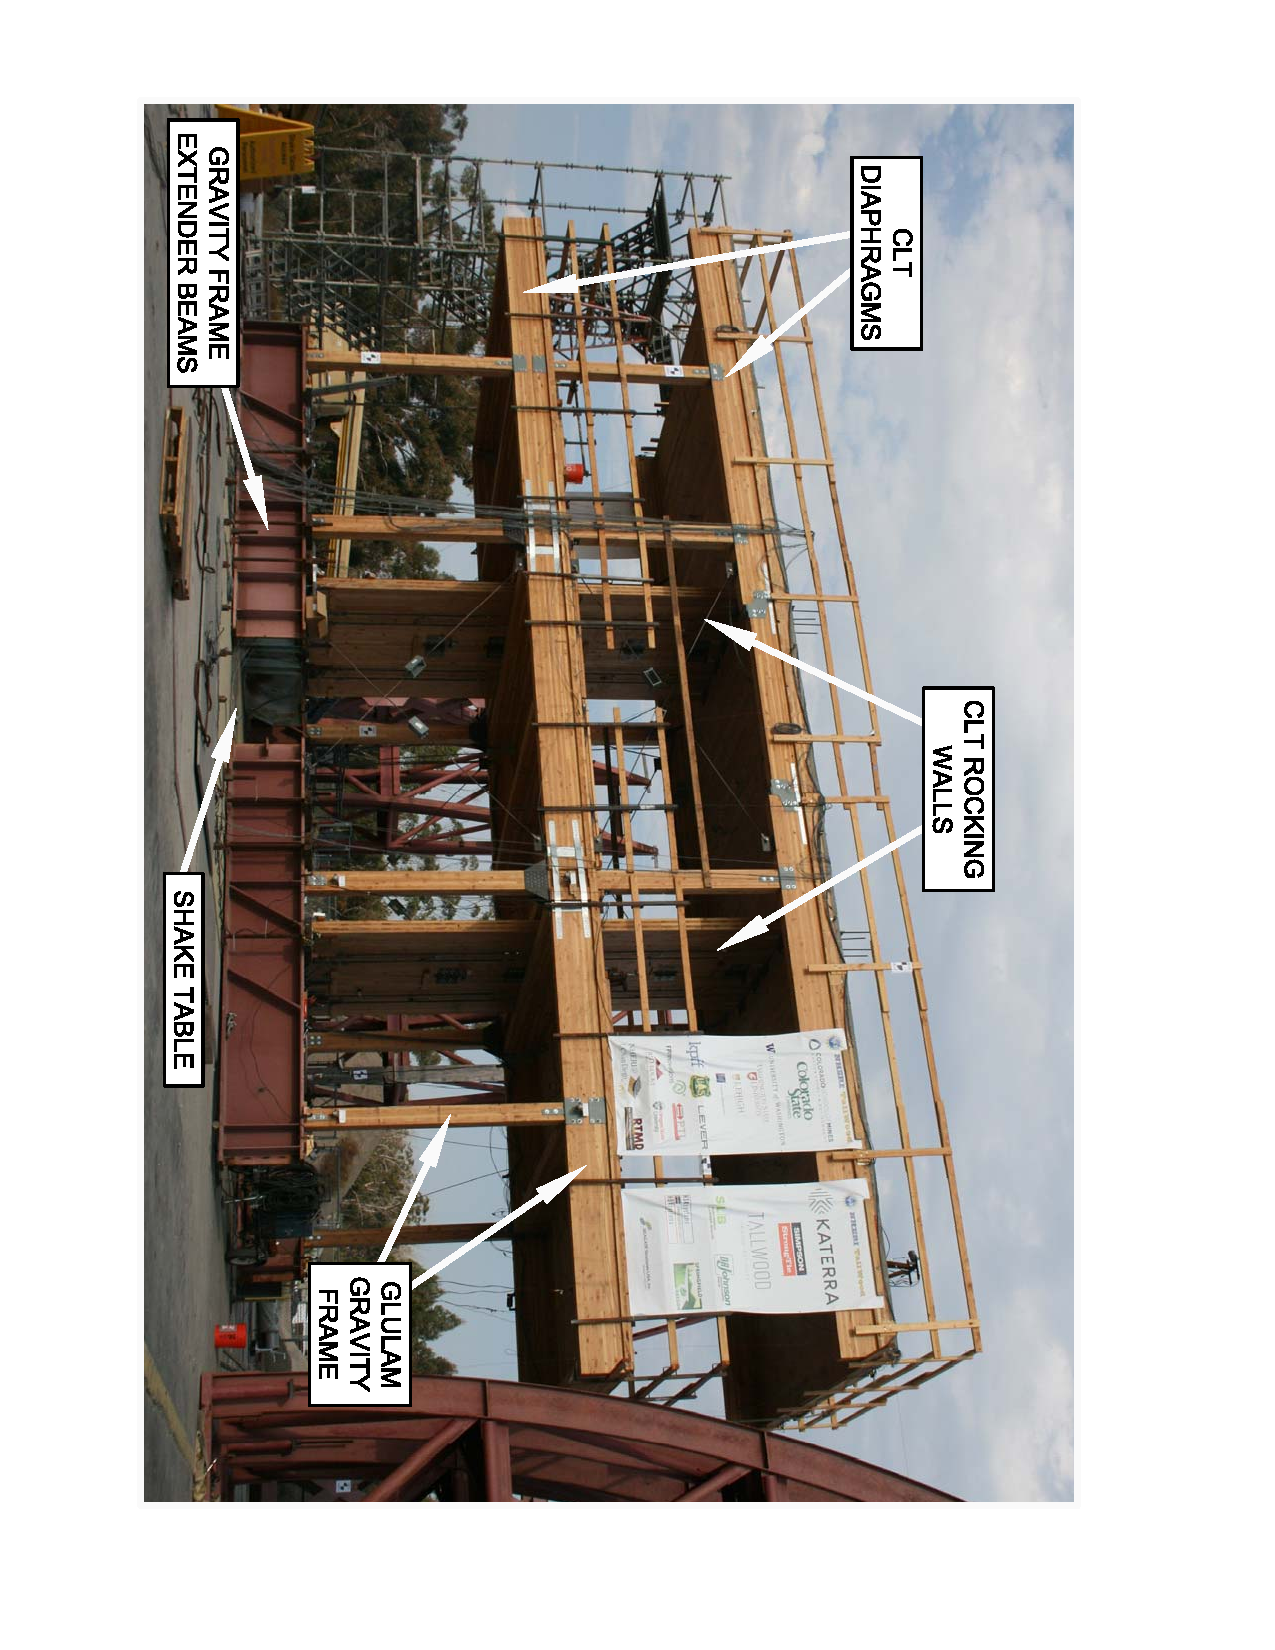
\includegraphics[width=3in, angle = 90,trim = {1in 1in 1.25in 0.75in},clip]{buildingPhoto.pdf}}
    \qquad
    \subfloat[Design Configuration]{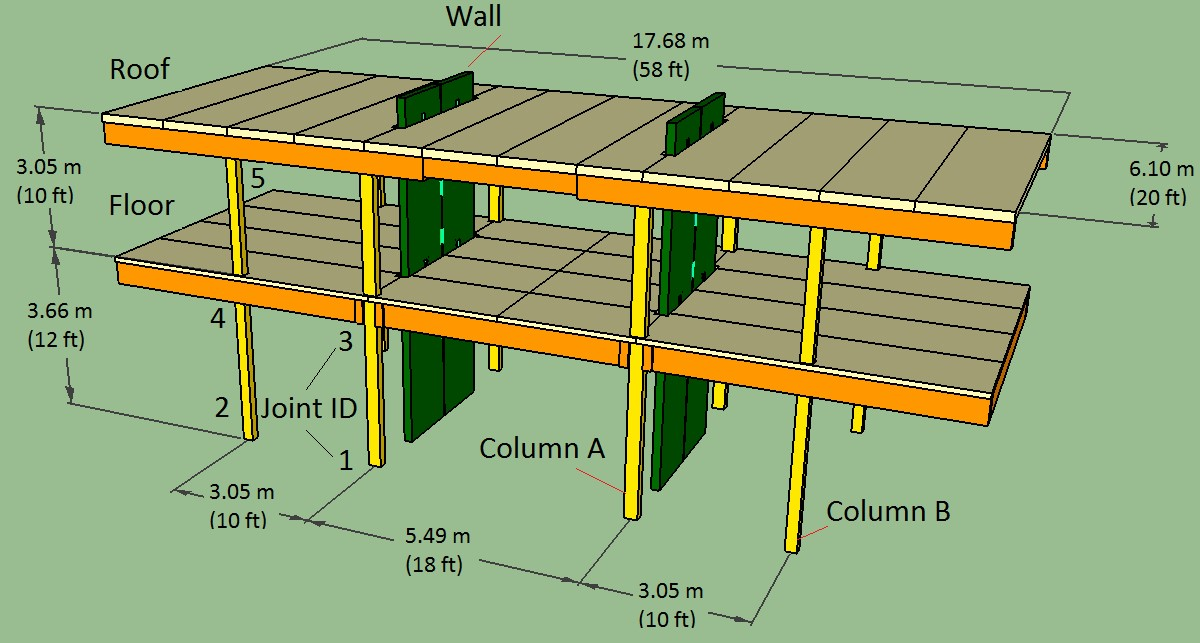
\includegraphics[width=4.5in]{sketchUpStructure.jpg}}
    \caption{Test Specimen \cite{Wichman}}
    \label{fig:Building}
\end{figure}

\subsection{Test Setup}

Fig.\  \ref{fig:Building} shows the structure tested. The test specimen was two stories, each with a floor size of 20 feet x 58 feet. The first floor was 12 feet tall and the second floor was 10 feet tall. The gravity loads were supported by columns, and the lateral loads were resisted by two coupled rocking shear walls \cite{Wichman}, see Fig.\ \ref{fig:Building}. The specimen was constructed on the NHERI shake-table at UCSD and can simulate ground motions in one direction. The specimen was constructed such that the ground motion would move in the direction parallel to the rocking shear walls.

\medskip

A series of fourteen total earthquake ground motions were used to test the specimen and in between the ground motions, white noise tests were completed to obtain the (elastic) natural period of the building. Table~\ref{table:schedule} summarizes all the tests and the order in which tests were completed. The tests are numbered 1-14 and are labeled based on the historic earthquake motion that they represent. The motions are also denoted as service level earthquake (SLE), design based earthquake (DBE), and maximum considered earthquake (MCE) these are indicators of the size of the earthquake. MCE are the largest earthquakes and SLE are the smallest earthquakes. More information about these earthquakes can be found in \cite{Wichman}. The white noise tests are denoted by WN. Again, they were run before and after every ground motion. Periodically during testing slight modifications to the structure were made, so white noise tests were also conducted before and after these modifications which is why two white noise tests sometimes happened right after each other as seen in the testing schedule. These modifications will not be discussed or analyses in detail in this report. In total there were 21 white noise tests. 

\begin{table}[!htb]
\footnotesize
 \centering
 \renewcommand{\arraystretch}{1.1}
 \caption{Testing schedule \label{table:schedule}}
  \begin{tabular}{| c | c|  c | }
  	\hline
  	\textbf{Day} & \textbf{Test} & \textbf{Motion} \\
  	\hline
  	\multirow{\textbf{Day 1}} &   & WN 1 \\
  	& 1 & Loma Prieta SLE \\
  	&   & WN 2 \\
  	\hline
  	\multirow{\textbf{Day 2}} &   & WN 3 \\
  	& 2 & Loma Prieta SLE \\\
  	&   & WN 4 \\
  	& 3 & Northridge SLE \\
  	&   & WN 5 \\
  	& 4 & Superstition Hills SLE \\
  	&   & WN 6 \\
  	& 5 & Northridge DBE \\
  	&   & WN 7 \\
  	\hline
  	\multirow{\textbf{Day 3}} &   & WN 8 \\
  	& 6 & Northridge DBE \\
  	&   & WN 9 \\
  	\hline
  	\multirow{\textbf{Day 4}} & 7 & Imperial Valley SLE \\
  	&   & WN 10 \\
  	& 8 & Northridge DBE \\
  	&   & WN 11 \\
  	\cline{2-3}
  	&   & WN 12 \\
  	& 9 & Loma Prieta DBE \\
  	&   & WN 13 \\
  	& 10 & Superstition Hills DBE \\
  	&   & WN 14 \\
  	\cline{2-3}
  	&   & WN 15 \\
  	& 11 & Loma Prieta MCE \\
  	&   & WN 16 \\
  	& 12 & Northridge MCE \\
  	&   & WN 17 \\
  	\cline{2-3}
  	&   & WN 18 \\
  	& 13 & Superstition Hills MCE \\
  	&   & WN 19 \\
  	\cline{2-3}
  	&   & WN 20 \\
  	& 14 & Northridge MCEx1.2 \\
  	&   & WN 21 \\
  	\hline
  \end{tabular}
\end{table}
\FloatBarrier

A total of 357 instruments were used on the structure for data collection. In this report only 24 of the acceleration sensors were used for the data processing. The sensors used were all 4000A Silicon Mems accelerometers with a full range of 10G from measurement specialties and had an accuracy of 5\%. Ten of the accelerometers used were located on the roof of the structure and another 10 were located on the first floor. Fig.\  \ref{fig:Accels} shows an aerial view of the floors with the locations of each accelerometer and their names labeled. Although the shake table only moved in one direction, at each location there were accelerometers that measured movement in each of the horizontal directions to capture any potential torsional effects in the building. The final four accelerometers that were used for this report were located at the base of each of the four shear walls and measured acceleration in the direction parallel to shaking. These four accelerometers were assumed to measure the movement of the shake table itself. 

\begin{figure}[!htbp]
    \centering
    \subfloat[First Floor]{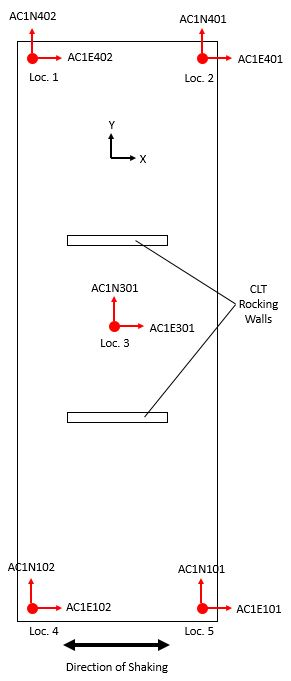
\includegraphics[scale = 0.8]{FloorAccel.JPG}}
    \qquad
    \subfloat[Roof]{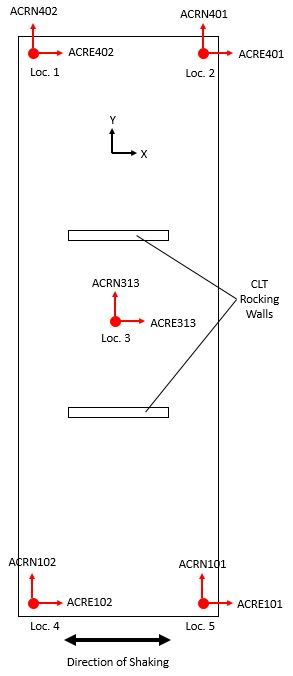
\includegraphics[scale = 0.8]{RoofAccel.JPG}}
    \caption{Aerial View of Accelerometer Locations and Names}
    \label{fig:Accels}
\end{figure}

\FloatBarrier
\subsection{Project Scope}

Due to the size of the test from which this data was collected, there was a lot of noise that appeared in the data. In order to begin data processing, all the acceleration data was first filtered using Gaussian filters in order to get more clear results. Both a high-pass and a low-pass filter were applied to the data. This processed data was then used for all the analyses discussed in this report. 

\medskip
As mentioned previously, White noise ground motions were used to excite the structure in order to capture the natural frequencies of the structure after each test/modification. The data obtained from the accelerometers were analyzed using Fourier transform to compute the dominate frequencies. The data was filtered through (1) Gaussian filter on the spectral content, and (2) averaging the spectral content from all the pertinent sensors. The natural frequencies of the first and second mode were computed. Moreover, the change in the frequencies due to the different tests/modifications was also explored.

\medskip 
Spectrograms were computed from accelerometer data from the structure excited by earthquake ground motions. This allowed the evolution of the frequency content to be visualized. The spectrogram also allows for comparison between low frequency and high frequency with respect to time and intensity of ground shaking.

\medskip
In addition, a modal analysis study was conducted on the overall structure to determine the primary modes of shaking. This was completed using a Single Value Decomposition (SVD) algorithm on filtered acceleration data in both the direction of shaking and the direction perpendicular to shaking. The results from the SVD were used to plot the primary modes of the structure. Finally, a low-rank reconstruction of the data was performed to determine how the data was affected by only accounting for the primary modes. 

\medskip
The last thing investigated with this data was an analysis of the interstory response. Data was taken in the principle ground motion direction (x-direction, shown in Fig.\  \ref{fig:Accels}) from all accelerometers on each story, and average time histories for each floor were extracted. An SVD of these time histories was completed, and a Fast-Fourier Transform of the primary mode revealed the fundamental frequency of vibration of each single-degree of freedom representation of the structure's floors. An observation matrix containing all story accelerations for each test in the x-direction was also investigated.

\FloatBarrier
%  Theoretical Background
\section{Theoretical Background}

\medskip
\textbf{\begin{center}Fast-Fourier Transform\end{center}}

\par Fourier introduced the concept of representing a given function $f(x)$ by a trigonometric series of sines and cosines: \\
\begin{center}$f(x) = $\sum_{{-}\infty}^{\infty}$ \frac{c_{n}e^{in\pi}}{L} \ \ x \in [{-L}, L]$ \\\end{center}
\par Based on this idea, the Fast Fourier Transform (FFT) was created, which transforms a signal from it’s
original domain to a frequency domain. The Fourier Transform is an integral transform defined over the entire line $x \in [− \infty, \infty]$. The Fourier transform and its inverse are defined as \\ \begin{center} $F(k) = \frac{1}{\sqrt{{2 \pi}}} \int_{{-}\infty}^{\infty}\ e^{ - ikx}f(x)dx      \ \ \    (13.1.8a,$ \cite{kutz_2013} $)$ \end{center}
 \begin{center}
$f(x) = {\frac{1}{\sqrt{{2 \pi}}}} \int_{{-}\infty}^{\infty}  e^{ikx}F(k)dk  \  \  \  (13.1.8b$
\cite{kutz_2013} $)$$\\ \end{center}
The key features of the FFT routine are as follows:
\begin{center}
\begin{itemize}
  
\item  It has a low operation count: \ $ O(N log N)$.\\
\item  It finds the transform on an interval $x \in [ {-L}, L]$. Since the integration kernel $e^{ikx}$ is oscillatory, it implies that the solutions on this finite interval have periodic boundary conditions. \\
\item  The key to lowering the operation count to $O(N log N)$ is in discretizing the range $x \in [ {-L}, L]$ into 2n points, i.e.\ the number of points should be [$2, 4, 8, 16, 32, 64, 128, 256, ...  $]. \\
\item  The FFT has excellent accuracy properties, typically well beyond that of standard discretization schemes

\end{itemize}
\end{center}
\par This type of transform can be used for many things in the field of digital signal processing and imaging because the transform can organize data by frequency and it can be easier to find strong frequencies and easier to identify frequencies that may just be noise. 
\textbf{\begin{center}Gabor Tranform/SFFT\end{center}}

\par We can easily obtain a Fourier transform of a set of points and resolve the frequency content of such a set; However, signals over time or space contain sets of points for each instance of the domain, and as a result, will lose the spatial or temporal resolution of frequency magnitude peaks within the signal once a Fourier transform is performed. This is due to the integration over the spatial or temporal domain which must be completed in order to resolve the magnitude of the frequencies of the signal throughout the domain. If the entire signal is sampled when a Fourier transform is completed, the frequency content of the signal’s entire domain is represented in the Fourier transform. 

\medskip 

One way to temporally localize peaks in the frequency of a signal is to utilize a window upon the temporal domain and perform a Fourier transform solely within the windowed domain. This way, the frequency content obtained from a spectral analysis of the window is known to most likely be within the window from which the frequency content was calculated. Sliding the window over the domain and performing Fourier transforms on the window creates spectral representations of each instance of windowing. These spectral analysis ‘slices’ can be plotted over time creating spectrograms to demonstrate the changes in frequency content throughout the signal. 

\medskip 

The chosen method employed here and described above is known as a Gabor Transform, a windowed version of the Fourier transform which involves replacing the original kernel of the Fourier transform with one that allows a window to slide over the domain of the function and isolate local frequency content centered around the window in time. What is described is a discrete form of the integral, \\\begin{center}
$G[f](t,\omega)=f(g (t,\omega))= \int_{{-}\infty}^{\infty}\begin\ f(t) g (\tau -t) \exp{(-i\omega t)} d\tau =(f,g\bar(t,\omega)))$ \end{center}\\ where the function f(t) represents the signal as it varies with time and $g (\tau -t)$ represents the Gabor Window which is utilized to filter the signal temporally. This can be represented in the following form, as found in \cite{kutz_2013}. \\

\begin{center}$f\widetilde(m,\ n)\ =\ \int_{{-}\infty}^{\infty}\begin\ f(t)g_{m,n}\ (t)dt  = (f,g_{m,n}) $, where $g_m_,_n(t)\ = g(t\ -\ nt0)\ \exp{(-i 2 \pi m t \omega_0)} $ \end{center}

\textbf{\begin{center}Singular Value Decomposition\end{center}} \\

\par The Singular Value Decomposition, or SVD, is an incredibly powerful tool in linear algebra which can be used to examine the principle dynamics of data. The technique uses an expansion of the data into two bases to represent said data in diagonalized form, with principle components and energies recorded to allow for reconstruction of the data in a lower rank. 
According to Kutz, in Data Driven Modelling and Scientific Computing \cite{kutz_2013} , for any set of data $A^{m * n}$, the SVD makes diagonalization possible if the proper bases for the domain and range are used. Consider that since U and V are orthonormal bases in $C^{m * m}$ and $C^{n * n}$ respectively, then any vector in these spaces can be expanded in their bases. In short, what this means is that any matrix can be diagonalized with the SVD, as the method is not contingent on positive definiteness or symmetry of the matrix. The SVD of a matrix is guaranteed to exist; but the SVD does not necessarily guarantee that all dynamics within the system will be captured. Careful inspection of the modal decomposition of the data and energies associated with the proper orthogonal modes sheds light on the primary dynamics and hidden dynamic behavior. The multiple bases utilized in the SVD allow for decomposition of a symmetrized form of the data matrix, $A$.  

\medskip

The SVD can be performed with the following matrix operations, 

\begin{center}$A^T A = (U\Sigma V^* )^T$,\end{center}
\begin{center}$(U\Sigma V^*)= V\Sigma U^*$\end{center}
\begin{center}$U\Sigma V^* = V\Sigma ^2 V^*$  (15.1.79, \cite{kutz_2013})\end{center}

and\\
\begin{center}$AA^T  =(U\Sigma V^* )$, \end{center}
\begin{center}$(U\Sigma V^* )^T=U\Sigma V^*$,\end{center}
\begin{center}$V\Sigma U^*  = U\Sigma^2 U^*$ (15.1.80, \cite{kutz_2013})\end{center}

Post multiplication of the above results with V and U respectively provides self-consistent Eigenvalue problems, \\
\begin{center}$A^T AV = V\Sigma ^2$  (15.1.81a, \cite{kutz_2013}) \end{center}
and
\begin{center}$AA^T= U\Sigma ^2$  (15.1.81b, \cite{kutz_2013}) \end{center}

The above represents the decomposition of the data into its principle components and singular values, which can then be used to create low rank approximations of the data. By examining the singular values and the principle components and contributions of each principle component to the features of the data analyzed, we can make inferences about the driving dynamics of the data and interpret the effects of interactions between components of the data. 

\FloatBarrier
% Algorithm Implementation and Development

\section{Algorithm Implementation and Development}

\subsection{Filtering}

Due to the large scale nature of this test, the data collected was very noisy, so before doing any analysis on the data, it was filtered. To determine which frequencies should be filtered out, an FFT was performed to find the frequency content of the signal. Using the results of the FFT, a Gaussian filter was chosen to filter out very high frequency data: 

\begin{equation}
    G(k) = \exp{(-0.008(k)^{2})}
\end{equation}

After looking more closely at the data, it was determined that there was also some very low frequency content that needed to be filtered out. In order to filter out this low frequency data, an inverted Gaussian filter was chosen: 

\begin{equation}
    G(k) = 1-\exp{(-1(k)^{2})}
\end{equation}

The data that resulted from using both these filters is what was used for all the analyses presented in this report. The same Gaussian filters were used for all accelerometer sensors on the structure. 

\subsection{White Noise} \label{Alg:WhiteNoise}

To obtain the natural frequencies from the white noise test, the accelerometer data (in the primary direction of shaking) from all 21 white noise tests were loaded into Matlab. Two for-loops were used, one to loop through each test (outer loop), and another to loop through each sensor (inner loop). Within the inner loop, FFT was computed on the filtered acceleration data. Then, the average of the filtered FFT data from the sensors are computed. The max value is identified with the max(abs()) function and the associated frequency is extracted. Note that the dominant frequency was extracted from the averaged data, and for each individual sensor as well. Next, the outer loop will repeat these steps for each test run. 

\medskip
In order to obtain the second natural frequency, the algorithm is repeated with a single Gaussian filter:
    \begin{equation}
        G(k) = 1- \exp{(-0.0002(k)^2)}
    \end{equation}
This is to prevent filtering out the second mode.

In summary, three data analysis tools were employed for this section: (1) Gaussian filter, (2) averaging filter, and (3) Fourier transform.

\subsection{Spectrogram of Ground Motion Response}

The algorithm for computing the spectrogram of the structure from the ground motion starts like the algorithm for the white noise. For the spectrogram, it is possible for higher mode effects to be removed using the Gaussian filter, thus only an inverse Gaussian filter was used:
    \begin{equation}
        G(k) = 1- \exp{(-1(k)^2)}
    \end{equation}
Note that the spectrogram was computed on data from a single sensor (center location on the roof) from test 14 (earthquake ground motion).

\medskip

In order to obtain the spectrogram, the Gaussian filter with a window size, and step size was selected (1 and 301, respectively). Then, the algorithm loops through each slice of time and filters the signal. Next, FFT was computed on the time filtered signal and saved into a matrix that contains all the frequency content for each time slice. Lastly, said matrix is plotted with time as the x-axis, and frequency as the y-axis.

\subsection{Modal Analysis of Structure}

Using the filtered acceleration data from test 14, an SVD was performed to extract the mode shapes. For this analysis the 20 accelerometers seen in Fig.\ \ref{fig:Accels} were all used. As row vectors, the data from each accelerometer was appended in one large matrix, and the SVD was taken of this matrix (using the built in SVD function in MATLAB). Careful consideration was taken when assembling this matrix and the order in which the accelerometer data was stacked in the matrix was noted. The order in which the matrix was assembled was as follows: 
\begin{equation}
    A = \begin{bmatrix}
    x_{floor1} \\
    y_{floor1} \\
    x_{floor2} \\
    y_{floor2} \\
    ... \\
    x_{Roof4} \\
    y_{Roof4} \\
    x_{Roof5} \\
    y_{Roof5} 
    \end{bmatrix}
\end{equation}
where $x_{floor1}$ is the filtered acceleration data in the x direction, on the floor, in location 1. Taking the SVD of matrix $A$ diagonalized the matrix and gives the lowest rank possible. Computing the SVD of the matrix $A$ results in three new matrices: $U$, $\Sigma$, and $V$. The matrix $U$ has all the modes in column vectors, in order of highest mode to lowest mode. The matrix $\Sigma$ shows how much variance is in each mode for each data point included. The matrix $V$ is a representation of how much each data group is projected onto each mode. 

\medskip

The amount of energy from each mode was calculated using the $\Sigma$ matrix. The diagonal of the $\Sigma$ matrix was divided by the sum of the diagonal to get the values in terms of percentage. To determine what each mode looked like, the $U$ matrix was used. This $U$ matrix shows for each mode, where the location of each data group would be. In order to visualize these modes better, the location of each accelerometer was plotted on a 3D plot. Then, for each mode, the mode shape value for each accelerometer location from the $U$ matrix was added to the original location. During this process, the data from the $U$ matrix that corresponded to the x direction accelerometer resulted in movement in the x direction for that mode shape and same for the y direction. In order to make the mode shapes more visible when plotting, a scale factor of 10 was applied to the displacements.

\medskip

A low rank reconstruction study was also performed on the data to determine how reconstructing the data to include only the first few major modes would affect the accuracy of the data. This was done by trimming the matrices $U$, $\Sigma$, and $V$ to only include the first few modes and then multiplying them together with $U\Sigma V^{*}$ to get the reconstructed low rank approximation of the data. 

\subsection{Interstory Response}

Average time history of story accelerations for Test 14 were extracted from summing over several realizations of filtered accelerometer data from each floor. A Proper Orthogonal Decomposition (POD) of the modes of the average accelerations per floor was examined, and an interpretation of the $U$, $\Sigma$, and $V$ components output from the SVD was made. The most powerful spectral content of the average story acceleration time histories was then investigated, and a correlative relationship between system dynamics and fundamental frequency of POD modes is proposed.

\medskip

Interstory response was investigated by examining the time history difference between accelerations at the base of the wall and the first story, and the difference between accelerations at the first story and those of the roof in the x-direction (primary direction of excitation). Nominal acceleration time history per story was determined by averaging over the time-synchronized accelerometer data of the groups of sensors on each level, effectively smoothing out some of the high frequency noise within the signal. A SVD was then completed on a set containing the average acceleration time history for each level of the structure. The primary modes of this SVD represent the largest variations in oscillatory behavior between stories over time. A Fourier Transform was then performed on the most powerful SVD modes representing interstory acceleration variance, and the most energy dense frequency of the spectral content was determined. 
\par In short, the algorithm can be described as follows:\\
\item 
    \begin{enumerate}
      \item For All Stories
      \begin{enumerate}
        \item[]% Empty item (nesting kept)
        \begin{enumerate}
          \item Filter Acceleration Data
          \item SVD of Acceleration Data by Story
          \item Perform FFT on most powerful U*S Reconstructions
          \item Extract Most Energy Dense Frequency
          \item Interpret, Store Results
        \end{enumerate}
      \end{enumerate}
  
      \item Create Interstory Acceleration Time Histories 
      \item Assemble Array of Interstory Acceleration T/H's
      \begin{enumerate}
        \item[]
        \begin{enumerate}
          \item SVD of Interstory Acceleration T/H Matrix 
          \item Perform FFT on most powerful $U*S$ Reconstructions of Interstory Acceleration
          \item Extract Most Energy Dense Frequency
          \item Interpret Results
        \end{enumerate}
      \end{enumerate}
    \end{enumerate}


\FloatBarrier
% Computational Results
\section{Computational Results}

\subsection{Filtering}

Fig.\  \ref{fig:filter} shows an example of the filtering procedure used for all the acceleration sensors. This figure shows an example of just one acceleration sensor, but the same process was used for all sensors. The top figure shows the frequency domain of the signal with the two Gaussian filters applied to remove the very high frequency content and the very low frequency content. The middle figure shows the post-processed frequency content, and the bottom figure shows a comparison of the unfiltered data with the filtered data. From this bottom figure it is clear that the signal is much clearer but still retains the general behavior. 

\begin{figure}[!htb]
    \centering
    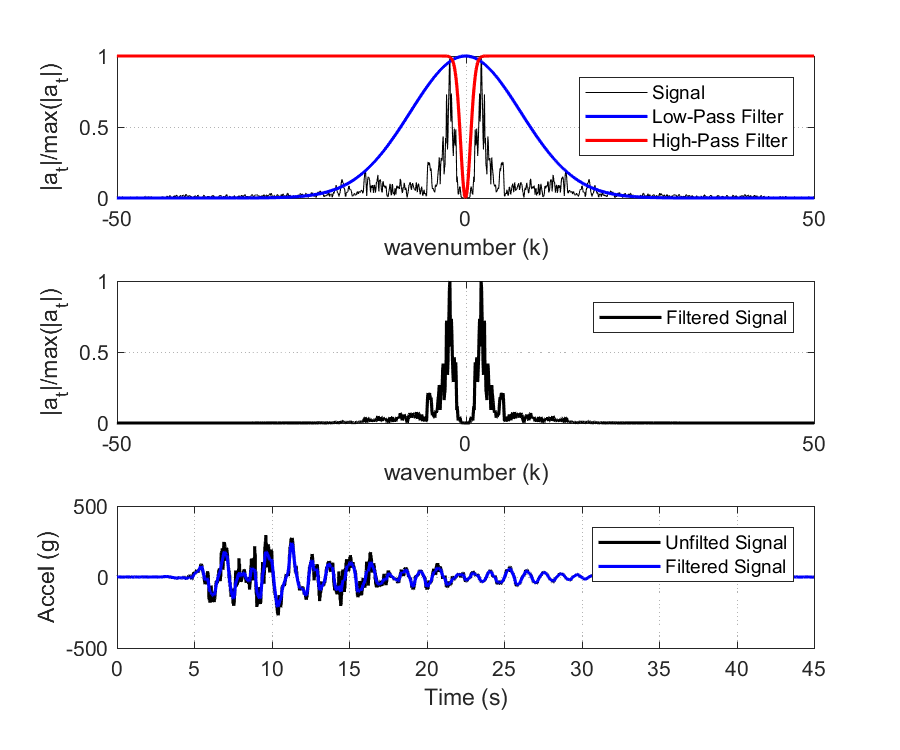
\includegraphics[scale = 0.7]{filter_ACRE313.png}
    \caption{Example of filtering procedure used. (Top) Signal in the frequency domain along with the two Gaussian filters used. (Middle) The post-filtered signal field in the frequency domain. (Bottom) The time domain reconstruction of the filtered signal field compared to the original, un-filtered signal}
    \label{fig:filter}
\end{figure}

\FloatBarrier
\subsection{White Noise}

Figure \ref{fig:First_nat_freq} shows the first natural period obtain from each sensor for tests 1, 2, 3, 7, 8, 9, 16, 20, and 21 (black circles). The blue line indicates the average of the black circles, and the red line is the first natural period using the average filter method (see Section \ref{Alg:WhiteNoise}). The agreement of the black circles for each tests indicates the Gaussian filter did a good job at cleaning up the noise. However, the discrepancy between the blue and red line, e.g.\ see Fig.\ \ref{fig:First_nat_freq} tests 3, shows that filtering via averaging reduced the noise further (noise that the Gaussian filter did not remove). Test 9 shows good agreement between the blue and red line, indicating the Gaussian filter removed most of the noise and the averaging filter did not contribute much.

\begin{figure}[!htb]
    \centering
    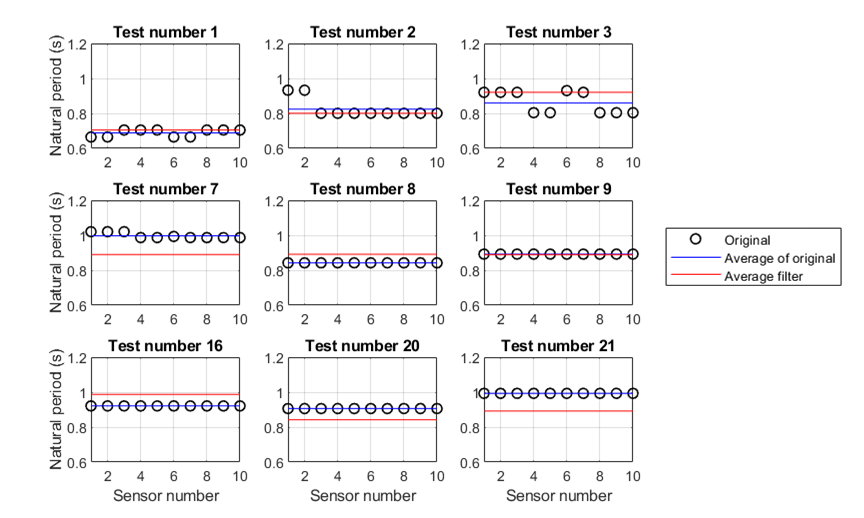
\includegraphics[scale = 0.7]{First mode frequency.png}
    \caption{First natural period}
    \label{fig:First_nat_freq}
\end{figure}

\medskip

By plotting the natural period from the individual sensors, the discrepancies from the sensors can also be identified. Lastly, the different tests yielded different natural periods. This is as expected because the white noise ground motion tests are performed between earthquake ground motion tests (and modifications) that may lead to damage or reparation of the structure, respectively. This can also be seen clearer in Fig.\ \ref{fig:Average_freq}. The natural period of the first and second modes are shown (top and bottom, respectively). The natural period of the first mode increases from tests 1 to 3. This is expected as test 2 was conducted after the first earthquake ground motion that likely loosen the structural connections (softening the system). Similarly, test 3 had an increase because the structure experienced yielding which further softened the system. The decrease in the natural period of the first mode can be contributed to reparations made to the structure.

\medskip

From Fig.\ \ref{fig:Average_freq}, there is not much variation in the natural period of the second mode. As expected, the natural period are lower for the second mode (higher frequencies). The consistency of the natural period of the second mode suggests that the higher modes are not sensitive to the structural damages incurred during earthquake ground motions.

\begin{figure}
    \centering
    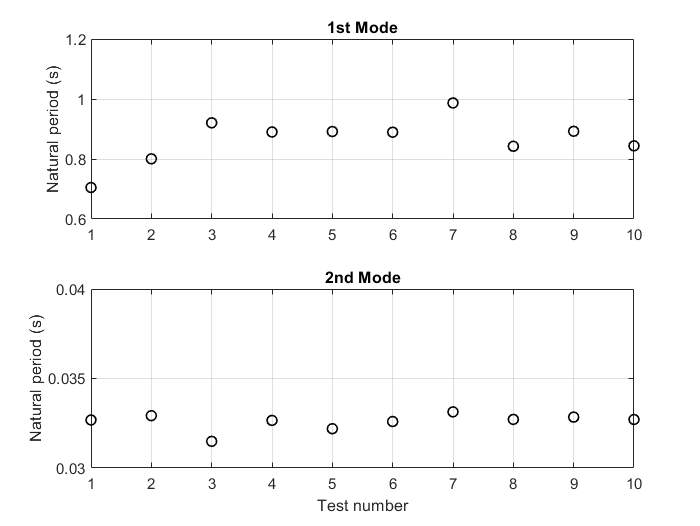
\includegraphics[scale = 0.5]{average_frequency.png}
    \caption{Evolution of first natural frequency}
    \label{fig:Average_freq}
\end{figure}

\FloatBarrier
\subsection{Spectrogram of Ground Motion Response}

Figure \ref{fig:Spectrogram} is a spectrogram of the acceleration from the center sensor on the roof from earthquake ground motion 14. Note that only data from this sensor from this ground motion was provided for the sake of brevity, but similar findings can be seen from the other data. 

\begin{figure}
    \centering
    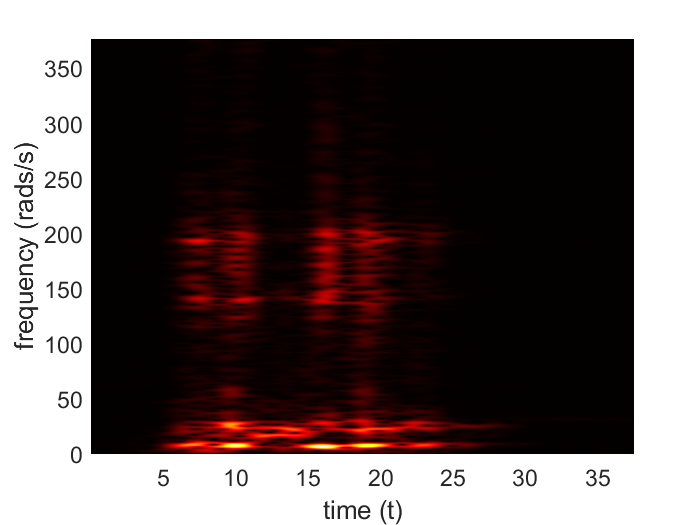
\includegraphics[scale = 0.55]{Spectrogram.png}
    \caption{Spectrogram of acceleration from ground motion 14, center sensor on roof}
    \label{fig:Spectrogram}
\end{figure}

\medskip

From the spectrogram, the signal noise is negligeable compared to the accelerations due to the ground motion, as expected. This can be seen by the lack of color before the 5 second mark and after the 30 second mark. The spectrogram illustrates the dominate frequency is approximately 8 rads/s. This is approximately 0.8 seconds, similar to the natural period from Fig.\ \ref{fig:Average_freq} (1st mode, test number 14). This is promising because it showed the structure primary response is similar to the natural period of the first mode. Furthermore, the higher frequencies shaking was present only during strong shaking. This can be seen from the spectrogram where high frequencies coincide with brighter colors in the lower frequencies. The higher band of frequencies (approximately 175 rads/s) is also around the natural period of the second mode (approximately 0.0325 s).

\medskip

The nature of earthquakes is that they occur in a wide range of frequencies (and often random-like features). As a results, the structure will respond with frequencies outside of the natural frequency. However, the structure acts similar to a filter in which the response is filter to the frequencies in the neighborhood of the natural frequencies of the structure.

\FloatBarrier
\subsection{Modal Analysis of Structure}

The results from this section are all from the data collected from test 14, the last and largest ground motion. The same analysis could have been done for any or all of tests, but only the results from one ground motion are included. Fig.\  \ref{fig:Energy} shows the amount of energy in each mode that resulted from the SVD test on the structure. The results from this plot show that the first mode is very much the dominate mode, accounting for almost 70\% of the total energy, which is very common for buildings and very much expected. The second mode accounts for about 20\% of the total energy and after mode 6, the energy contribution is near zero. 

\medskip

\begin{figure}
    \centering
    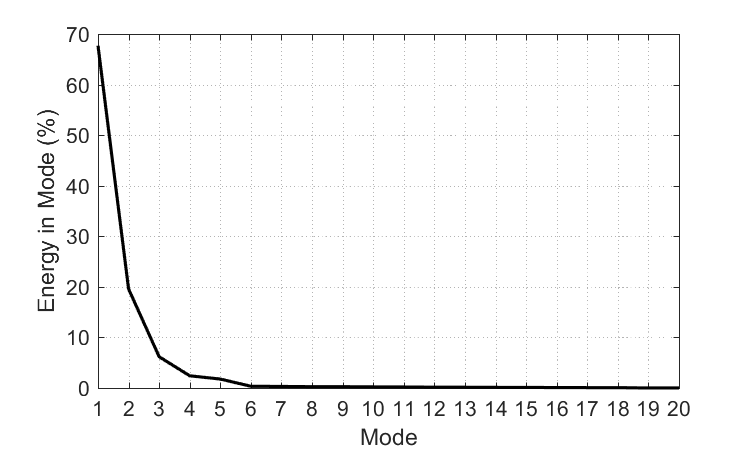
\includegraphics[scale = 0.7]{Energy.png}
    \caption{Energy per mode from the SVD analysis of the structure}
    \label{fig:Energy}
\end{figure}

Fig.\  \ref{fig:modes} shows the results of the $U$ matrix from the SVD. It should be noted that on the x axis are the nodes or the accelerometer recordings. Every other recording is the representative of the acceleration in the direction perpendicular to shaking, which is why most of them are near zero. We would expect that the first couple modes are primarily in the direction of shaking which is what we see for modes 1 and 2. It should also be noted that the first half of the points are representative of the accelerations recorded on the floor and the second half are from the roof. In the first mode, all movement is in the same direction, but for the second mode, the first floor goes in one direction while the roof goes in the opposite direction. This is expected behavior in buildings. The third mode doesn't have a clear pattern like the first two modes, so this is probably a torsional mode. 
\medskip

\begin{figure}
    \centering
    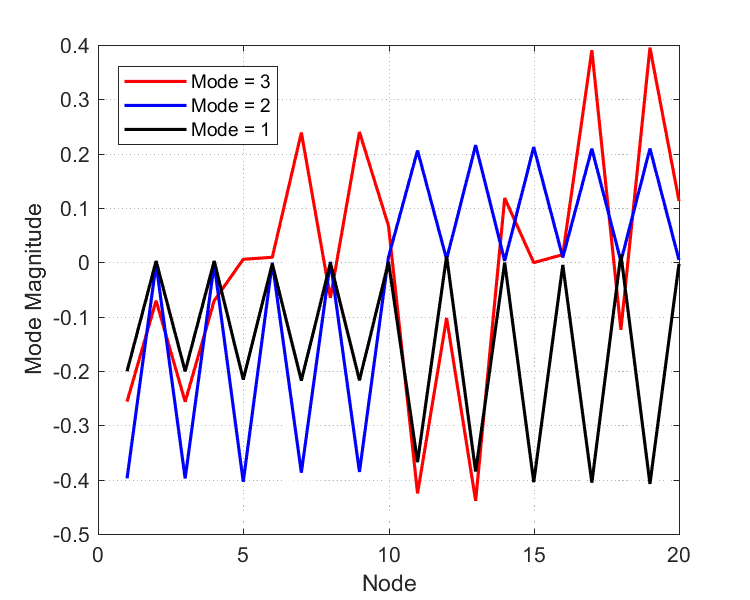
\includegraphics[scale = 0.7]{modes.png}
    \caption{Modes from the SVD analysis of the structure}
    \label{fig:modes}
\end{figure}
\FloatBarrier

To get a better visual idea of these  modes shapes, the mode values from Fig.\ \ref{fig:modes} were applied to the corresponding locations of the accelerometers and plotted as displacements in 3D. This visual representation of the mode shapes can be seen in Fig.\ \ref{fig:modes_shapes}. In these plots, the grey lines are representative of the original location of the floor and roof, while the black lines are the mode shapes. The first mode is exactly what we would expect in a building. Both the floor and roof move in the same direction that is also in the same direction as the earthquake shaking. The second mode is also what is expected. The roof has movement in one direction while the floor is moving in the other. The third mode shape is also what we predicted from Fig.\ \ref{fig:modes}: it is a torsional mode. The fourth mode is very similar to the first mode, but the movement of the floors is in the direction perpendicular to earthquake shaking. The following two modes are different types of torsional modes. These are all modes that we would expect for building response. It should be noted that only data from the floor and roof were used (no data from the wall was used) so these mode shapes are only representative of how the floors moved, not the walls. Future study can be conducted on the sensor data along the height of the wall that may lead to findings on higher mode effects that is not torsional but what is expected for higher modes of cantilever walls.

\medskip

\begin{figure}
    \centering
    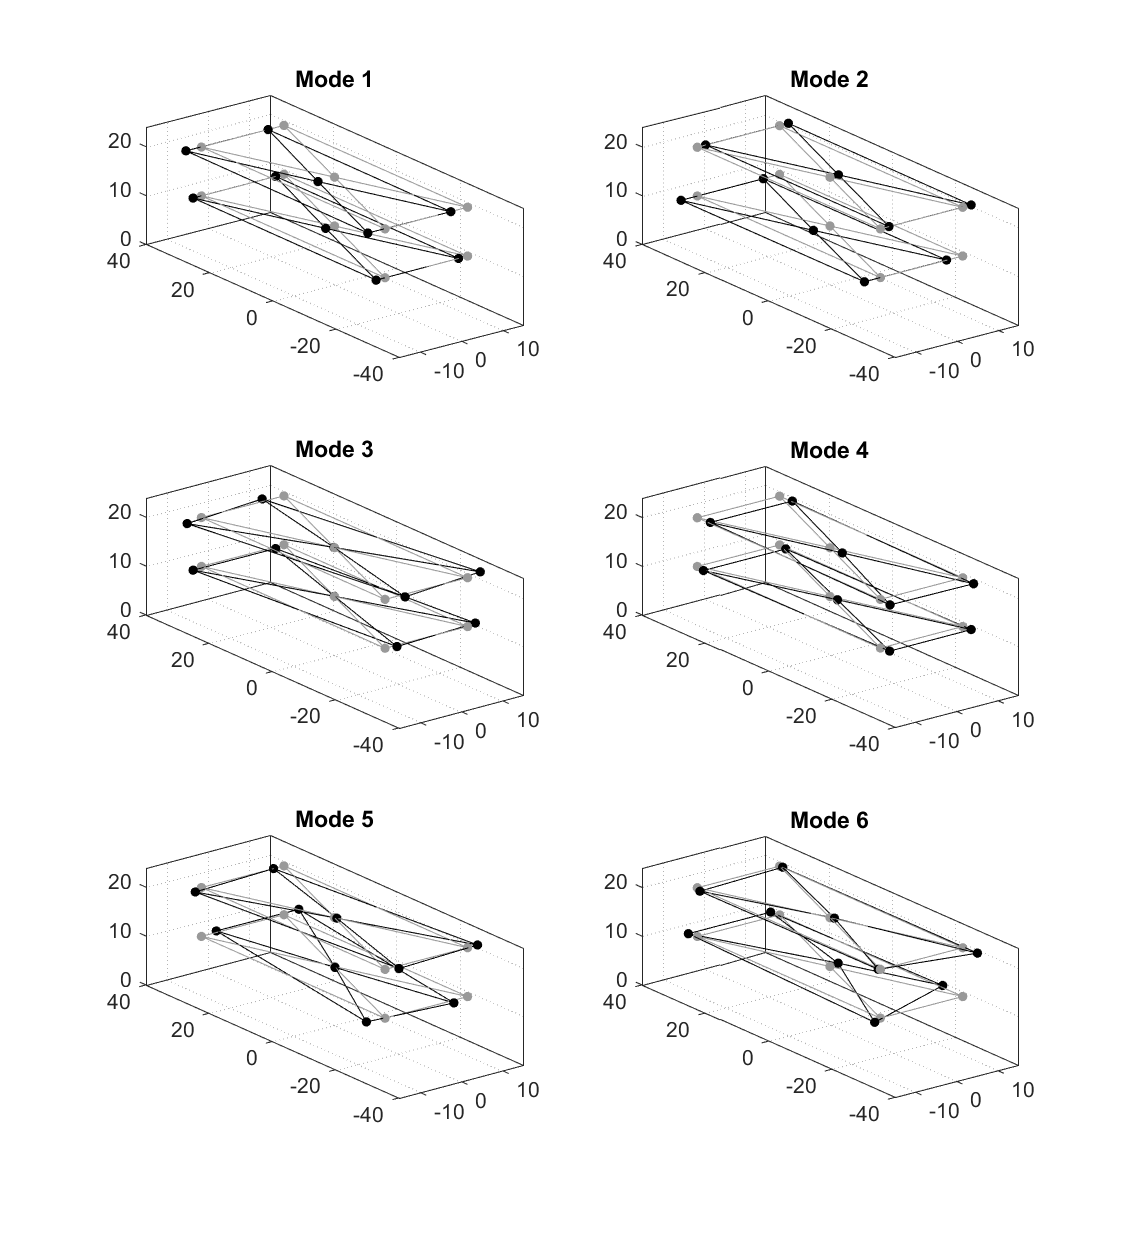
\includegraphics[scale = 0.8]{modes_shapes.png}
    \caption{Mode shapes from the SVD analysis of the structure}
    \label{fig:modes_shapes}
\end{figure}
\FloatBarrier

The final portion of the modal analysis was to complete a low-rank reconstruction. From Fig.\ \ref{fig:Energy} it is clear that anything greater than the second mode doesn't contribute much to the overall behavior. The low-rank reconstruction for two acceleration sensors are show in Fig.\ \ref{fig:reconstruction}. This figure shows a rank reconstruction of rank 1, 2, 5, and 10. The rank 2 reconstruction does a very good job at capturing the overall behavior. Because of this, we can conclude that there were very small torsional effects during the shaking of the structure, almost all of the movement was just from first and second mode effects.  

\begin{figure}[h]
    \centering
    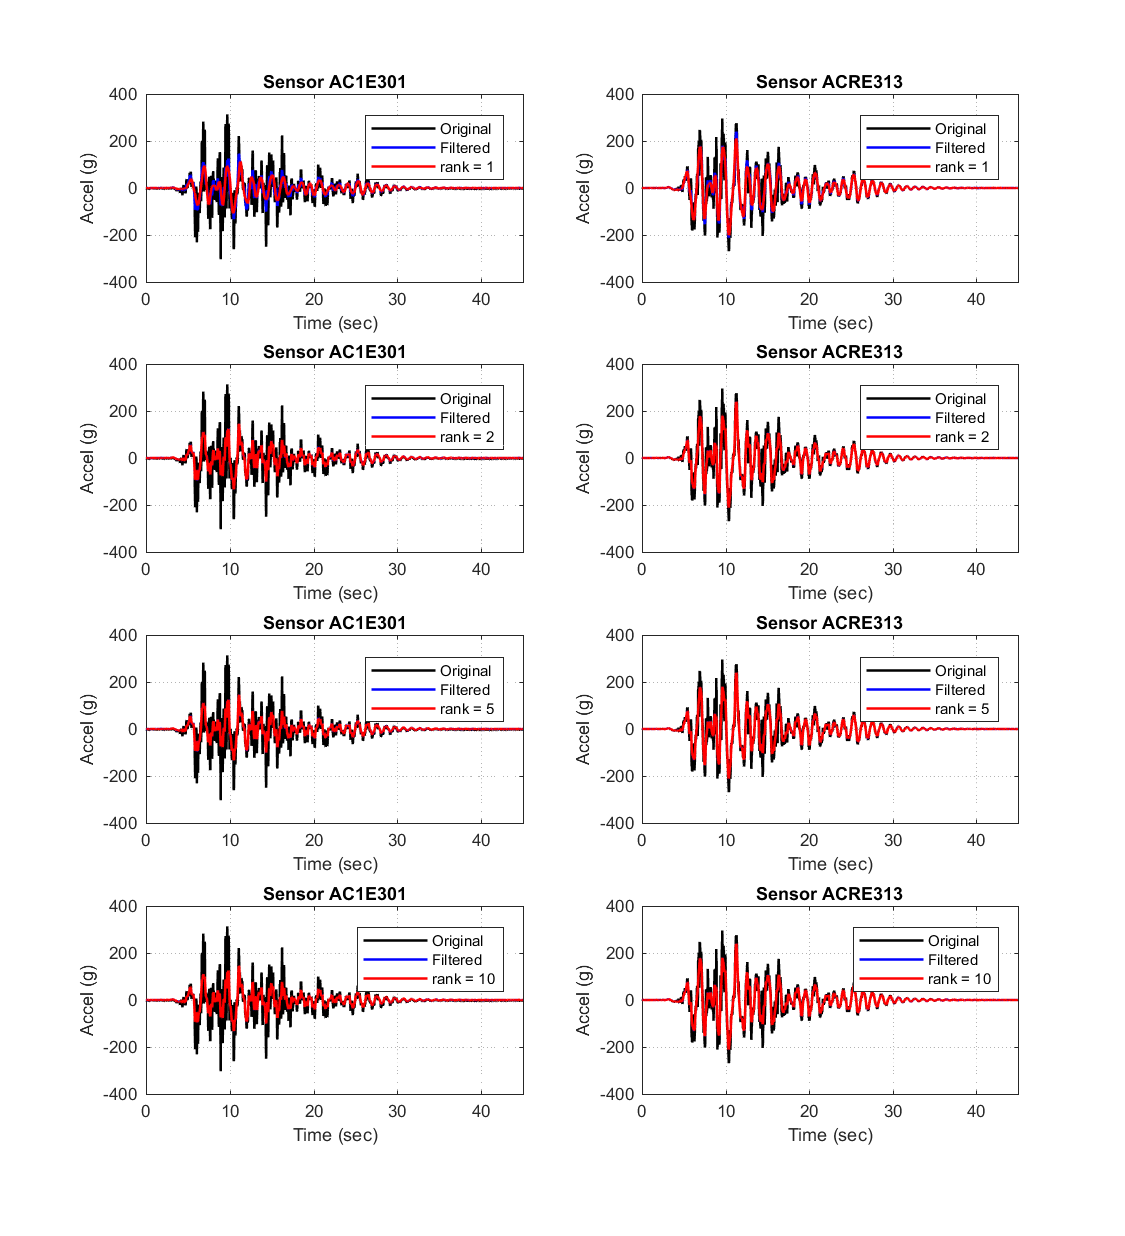
\includegraphics[scale = 0.8125]{reconstruction.png}
    \caption{Low-Rank reconstruction of the accelerometers from the SVD of the structure}
    \label{fig:reconstruction}
\end{figure}

\FloatBarrier
\subsection{Story/Interstory Response}

The first four modes from the SVD of the single degree of freedom accelerometer data seen in the left-most columns of Fig.\  \ref{fig:SVDFFTR} and Fig.\  \ref{fig:SVDFFTB}. 
As can be seen in Fig.\  \ref{fig:SVDFFTR} in the leftmost column, the average acceleration data (shown in red, underneath the most powerful reconstructed mode) lacks high degrees of noise, and the frequency content of the data indicates that there is a predominant frequency which contains most of the signal's energy. Other modes of the POD represent the dominant variations from the averaged signal that each measurement is somewhat likely to be partially comprised of. SVD modal participation is contained within $V$, however, the modal participations of an SDOF vibration is not of interest in this case. From the PSD plot on the right-hand side of the figure one can note the dominant power density of the primary frequency of pointwise vibration in the first POD mode, while the frequency content and power spectra content of the other modes is saturated and no dominant frequency is discernible. This indicates high congruence of the acceleration data measured from each of the sensors within the floor in the inspected direction, with little time variance and negligible amplitude/power difference.

\medskip

\par In order for frequency content of a single degree of freedom to be resolved, a Fourier Transform was performed on the time history content of the primary modes of the SVD. The results of the Fourier Transform and Power Spectral Density Estimates of the SVD modes can be seen in the centre and righthand columns of Figs.\  \ref{fig:SVDFFTR} through  \ref{fig:SVDFFTB}.
\begin{figure}[h]
    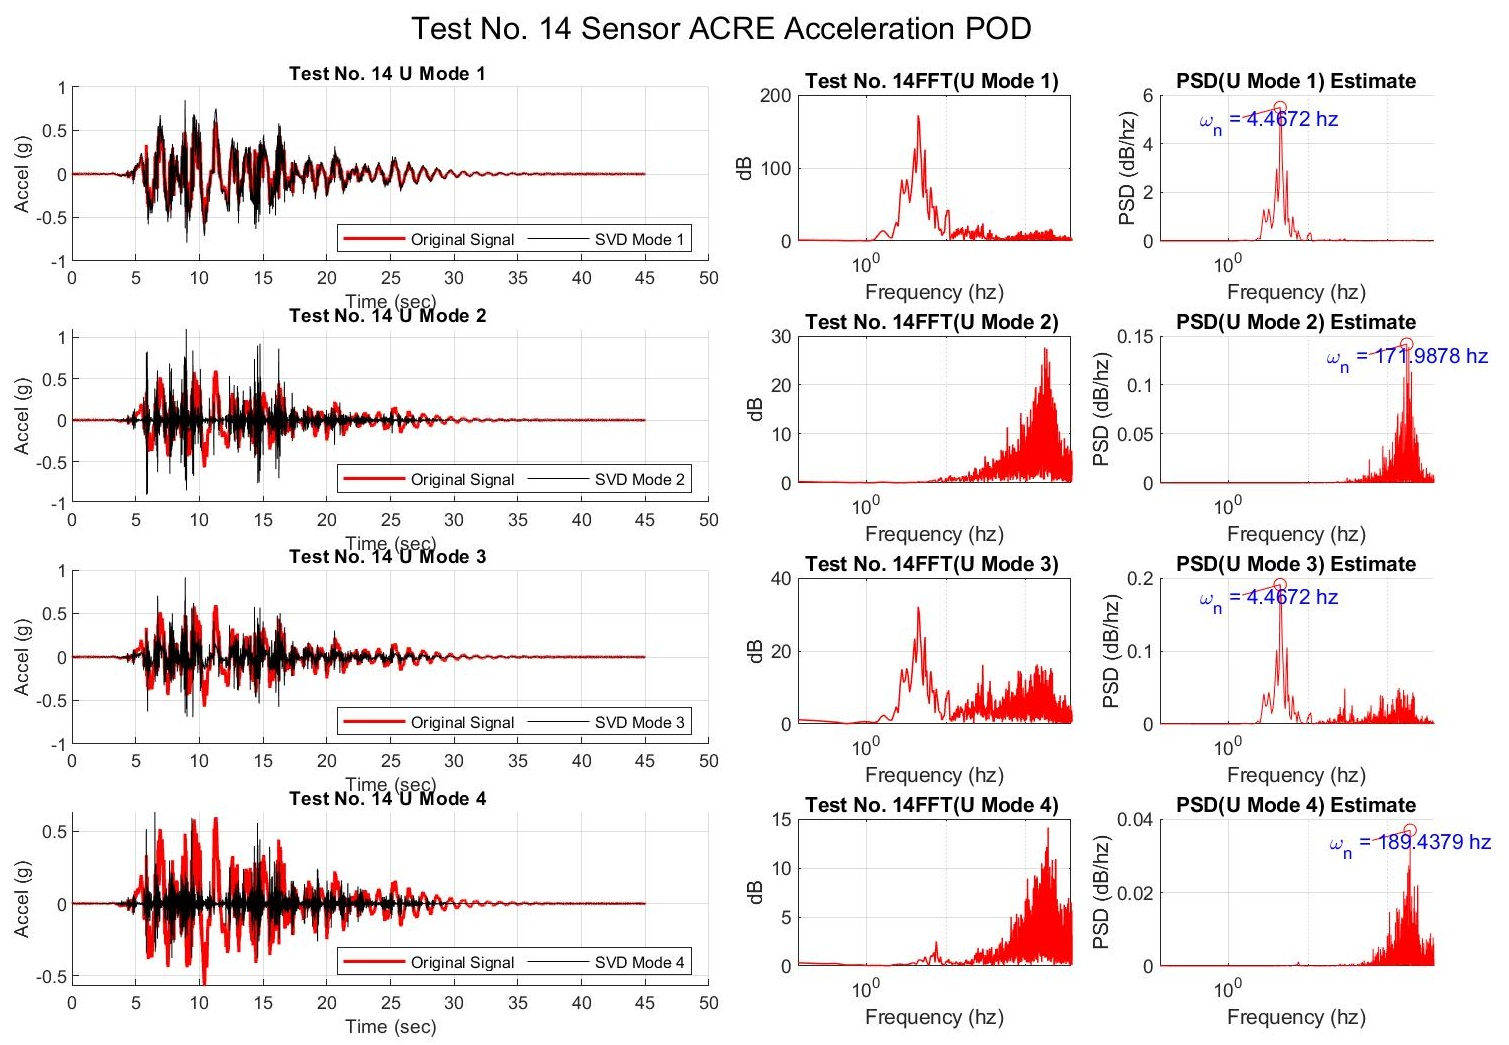
\includegraphics[width=1.05\textwidth,keepaspectratio]{Test14ACRE.jpg}
    \caption{SVD and FFT(U) of Roof Accelerations.}
    \label{fig:SVDFFTR}
\end{figure}
\\
\\
\par
The observation matrix for the SVD of the acceleration time history each floor contained all x-direction accelerometers for Test No.\ 14. Output and the SVD modes are comprised of variations between sensor acceleration magnitude measurements, key features of higher energy vibrations and shocks, and predominant excitation of modes of lower energy vibration. The most powerful mode of each SVD is evidently the transient and homogeneous vibrational response of the story to the ground motion excitation. Most of the vibrational energy of the system is captured by the first mode of the SVD (power scaling from the $S$ components of the SVD is represented by the projection of $U$ into the (g) domain via $U*S$). The second, third and fourth modes represent the predominant variations of signal intensity and phase from the average predominant  behavior of the  data set, as well as noise that is common to all signals. 

\medskip

\par 
Looking closely at the first and third modes of the SVD in Fig.\  \ref{fig:SVDFFT1}, there is a clear difference in the frequency concentration. The first mode is the predominant motion of the ground acceleration. The second most powerful can be interpreted as the contribution to overall acceleration the from action of the floors in tandem, synchronized aside from a slight change in phase. The third mode of the SVD can be interpreted as the effect of a secondary dynamical state, whether it be the second or third lowest energy mode of structural response vibration or a compound effect of several participating vibrational modes. 
\\
\begin{figure}[h]
    
    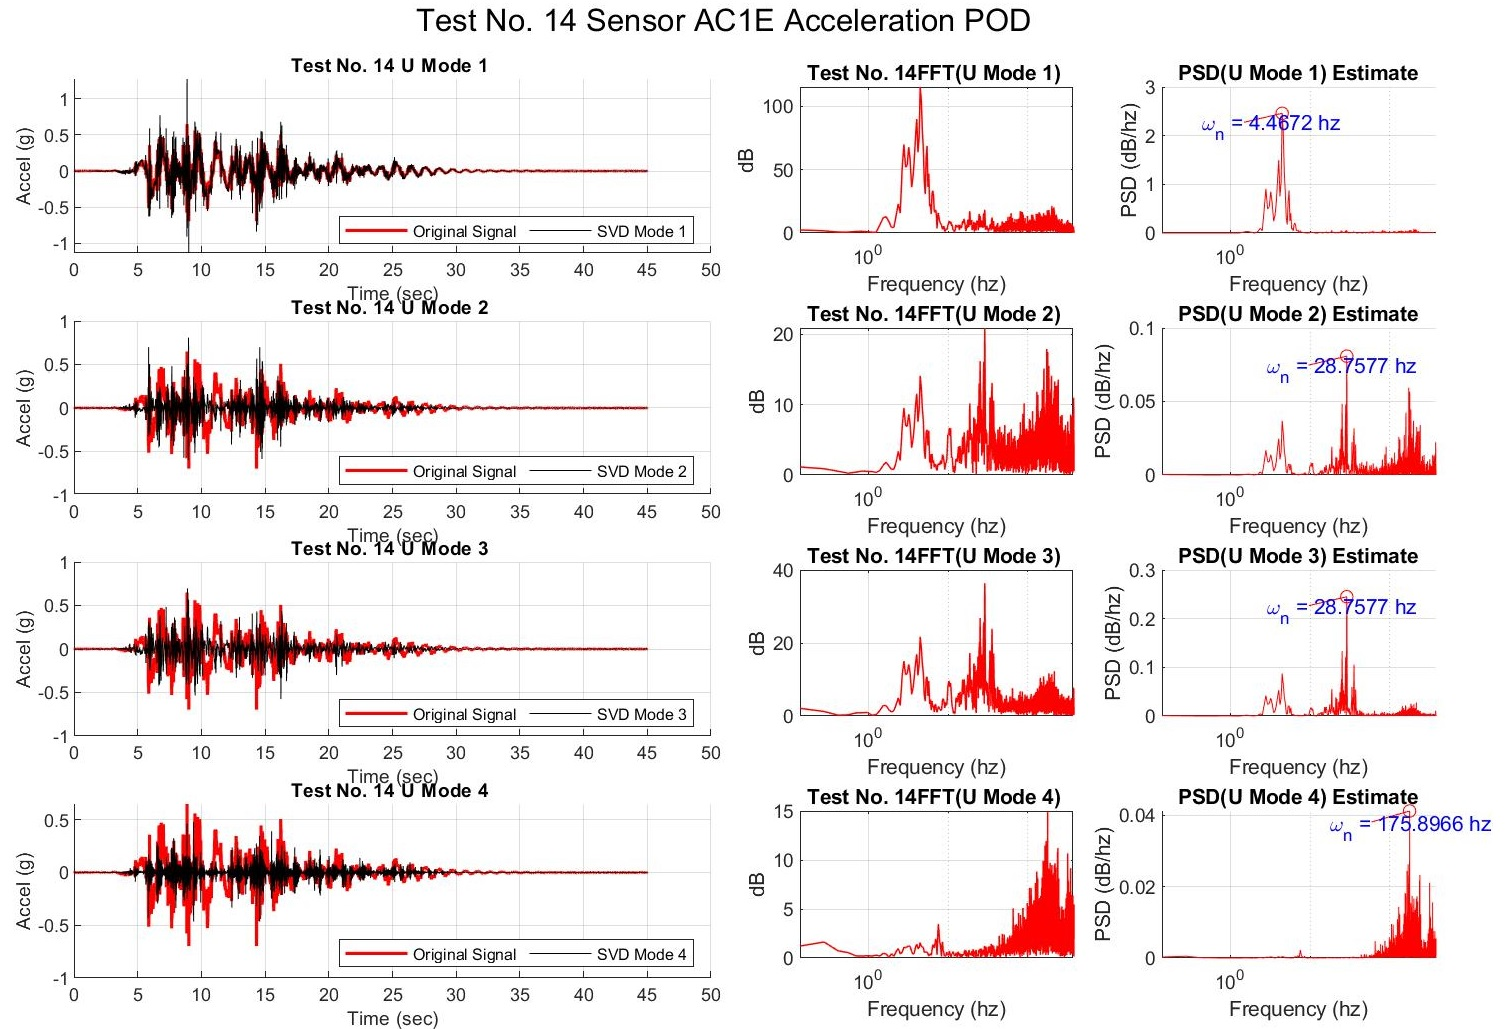
\includegraphics[width=1.06\textwidth,keepaspectratio]{Test14AC1E.jpg}
    \caption{SVD and FFT(U) of $1^{st}$ Story Accelerations.}
    \label{fig:SVDFFT1}
\end{figure}
\\
\\
\begin{figure}[h]
    
    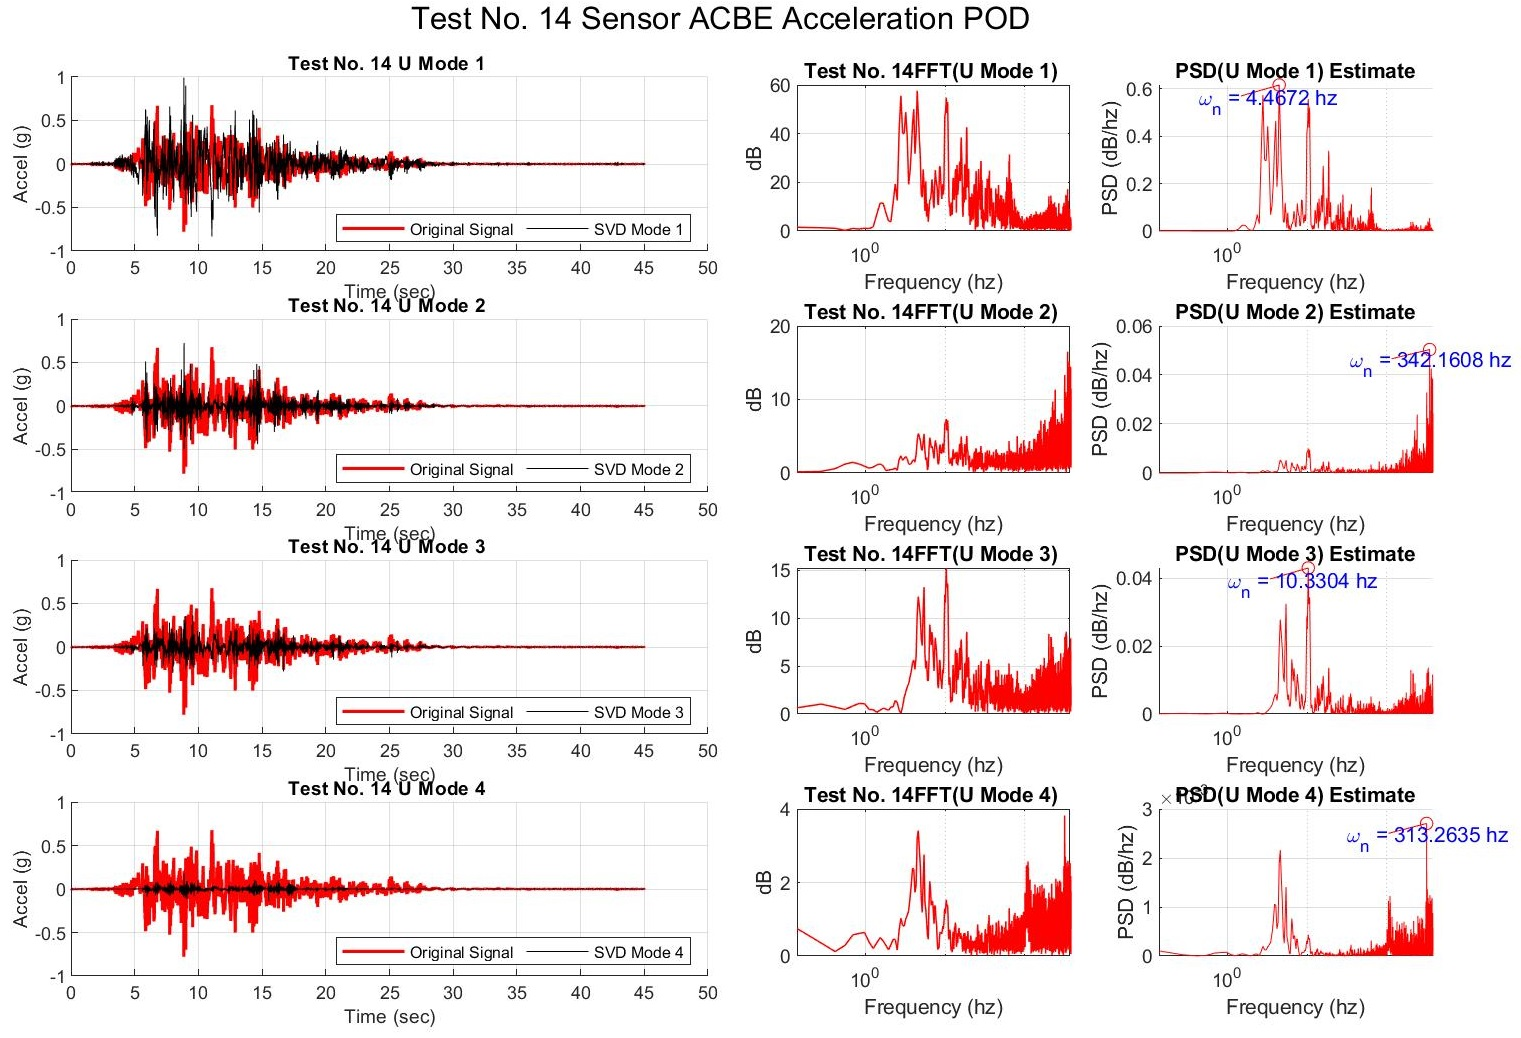
\includegraphics[width=1.06\textwidth,keepaspectratio]{Test14ACBE.jpg}
    \caption{SVD and FFT(U) of $1^{st}$ Story Accelerations.}
    \label{fig:SVDFFTB}
\end{figure}
\FloatBarrier

\begin{figure}[]
    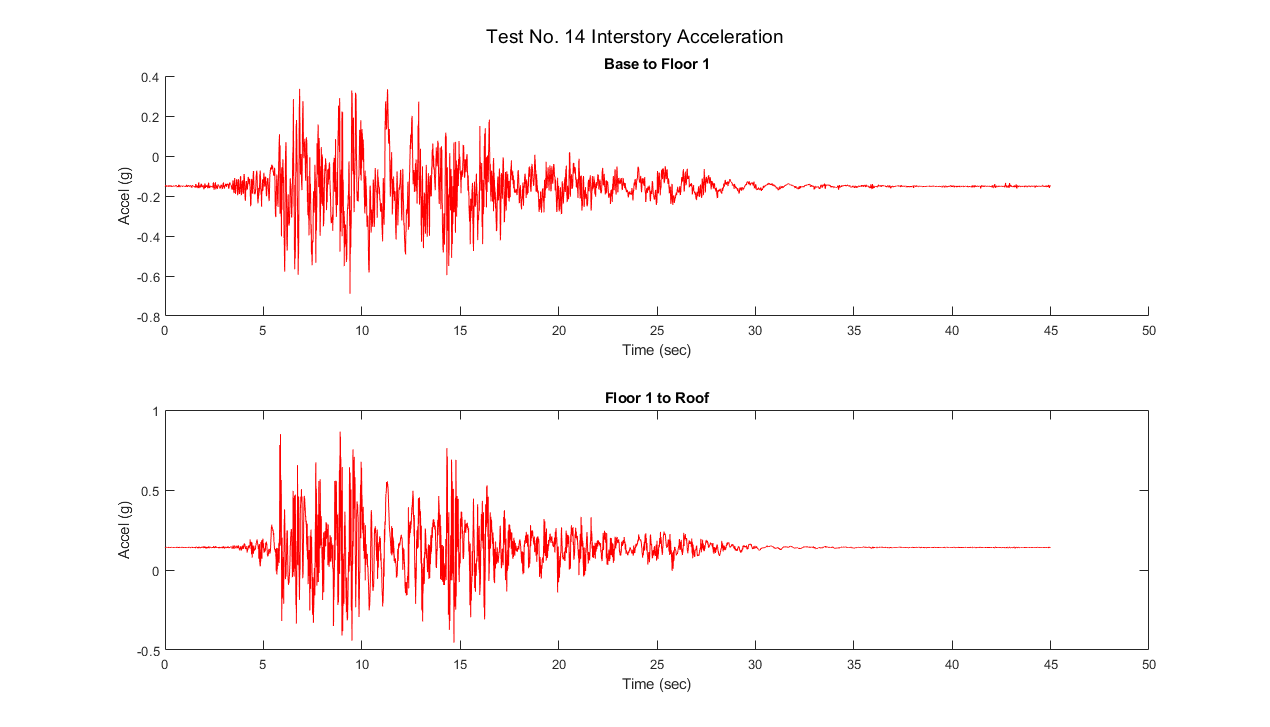
\includegraphics[width=\textwidth,keepaspectratio]{Test14_IA.png}
    \caption{Interstory Accelerations.}
    \label{fig:SVDFFT_IA}
\end{figure}
\begin{figure}[h]
    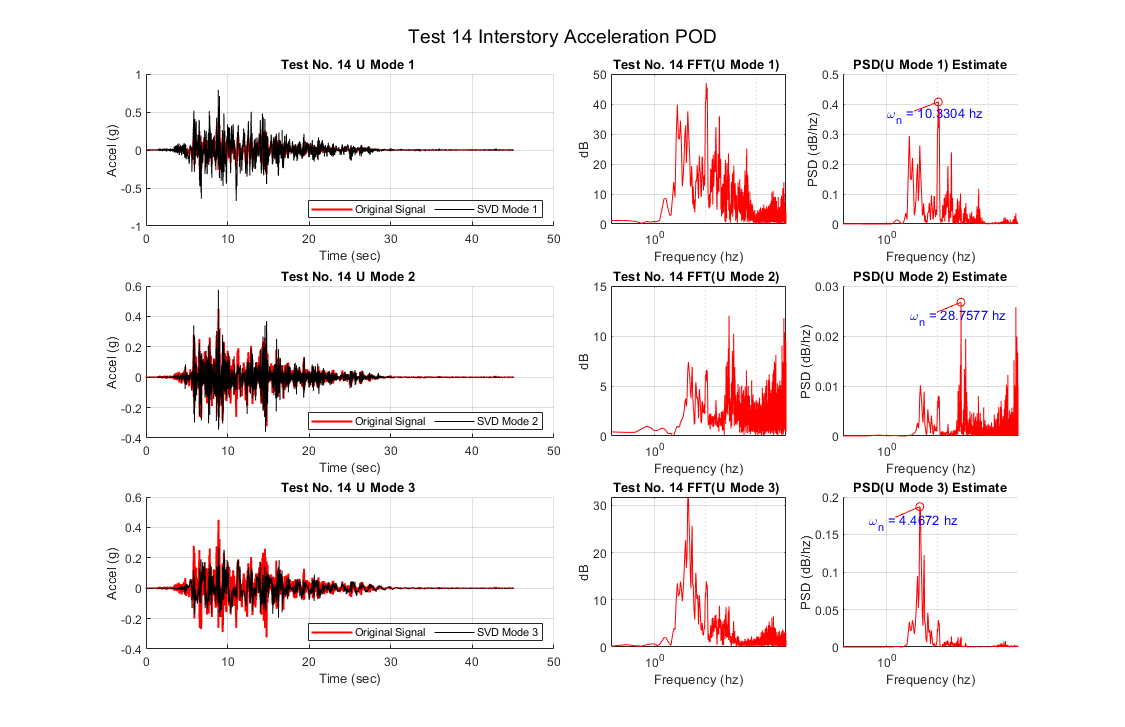
\includegraphics[width=\textwidth,keepaspectratio]{Test14.png}
    \caption{SVD and FFT(U) of Interstory Accelerations.}
    \label{fig:SVDFFT_fin}
\end{figure}
\FloatBarrier
\\
\\
\\
\par
Fig.\  \ref{fig:SVDFFT_IA} shows the interstory accelerations extracted from the averaged story acceleration time histories. The interstory relative accelerations between Floor 1 and the Roof are nearly two times those of the relative accelerations between the base of the structure and the first floor. This is likely due to combinations of first and second vibrational mode effects, their superpositions of modal vibration and shapes acting in constructive interference beats to generate larger amplitude accelerations within the second story portion of the shear walls. 

\medskip

\par A singular value decomposition of the averaged story acceleration time histories (base, $1^{st}$ floor, and roof) was completed and a Fourier analysis was completed on the strongest power orthogonal modes of the decomposition. The results of this analysis can be seen in Fig.\  \ref{fig:SVDFFT_fin}. 
The spectral analysis represents the fundamental frequency of the time history of variations in structural response acceleration between measurements at varying points along the structure's height due to random base excitation in the primary direction of resistance. The frequency of the ground motion was found to be roughly 4.46 hertz, and the natural frequency of the first most powerful resonance mode obtained from the singular value decomposition of the acceleration data from sensors in the ground excitation direction along various heights of the structure was $10.33 $hz, giving the structure a measured first natural period, $T_{nSVD1}$, of $0.6082$ seconds. 
The natural frequency of the second mode of the structure appears to be $28.757$ hz with measured second natural period, $T_{nSVD2}$, of $0.2185$ seconds. 

\medskip

\par This is incongruent with previously found values for the resonant frequency, which were obtained via pointwise investigation of the Fourier transform of the acceleration data of the individual sensors. What likely is happening with the SDOF extraction is a biasing of the Fourier domain toward the predominant ground motion acceleration frequency, as the acceleration data was not normalized by the ground motion acceleration and thus that ground motion frequency participated in the Fourier Transform. This would have an effect of lengthening the estimated period of vibration, which is in agreement with the postulation of ground motion acceleration biasing SDOF FFT output to lower frequencies, as the spectral content of the modes of the SVD of the interstory accelerations is of higher frequencies than that of the SDOF analysis. Since the ground motions are included in the SVD of the overall interstory acceleration data, they are easily extracted by the SVD as they are the most powerful contribution to acceleration, and the remaining most powerful modes of the SVD to be examined are either noise or dynamical response modes which can be isolated and analyzed for their frequency content, which possibly provides the overall structural dynamical response natural frequencies of the system.


\FloatBarrier
% Summary and Conclusions
\section{Summary and Conclusions}

Data from two-story timber building shake table test were analyzed to investigate the dynamical properties and the ground motion response of the structure. The accelerometer data was filtered using a Gaussian and inverted Gaussian filter in order to remove high frequency and low frequency noise.

\medskip

The data from the white noise test gave the natural period of the first and second mode (0.9 seconds and 0.0325 seconds, respectively). In addition, it showed the change in the natural period of the first mode between each ground motion testing and modification. The natural period of the second mode appeared to be less sensitive to the damage and modifications on the structure. From the consistency in the natural period from the individual sensor results, it can be seen that the Gaussian filter performed well. However, future study can further examine this by removing the filter and looking at the natural period from the individual sensor results (if the results remain unchanged, then that indicates the noise did not affect the results of the natural period). Furthermore, the discrepancy between the individual sensor results of the natural frequency and the natural frequency from the average filter method suggests that the average filter further reduced noise in the data.

\medskip

Spectrogram were computed and showed that the dominate frequencies are in the neighborhood of the natural period of the first mode. In addition, the frequencies from the higher modes were only present during intense shaking (and were also in the neighborhood of the natural period of the second mode). From this, it can be seen that the structure acted as a vibration filter which took the wide range of frequencies from the earthquake motion and responded with two frequency bands. The third and higher modes were not immediately visible from the spectrogram. Future study can compare the frequency content of the earthquake and compare it the frequency content of the structure's response.

\medskip

Modal analysis was done using SVD. Singular value decomposition was done on the sensors from test 14 and showed the energy of each mode
(70\% and 20\% for mode 1 and 2, respectively). The SVD also revealed that negligle energy was contributed by modes higher than 6.
The SVD also allowed the visualization of the mode shapes of the building, which were as expected from studies in earthquake engineering.
Low rank reconstruction was done and showed the dynamical behavior was mostly contained within the first two modes. Note that this is not how earthquake engineers typically get the mode shapes. Typically, eigen-analysis is used, but it is shown that SVD gives the same results commonly seen in earthquake engineering (or structural dynamics).

\medskip

The first mode of the Singular Value Decomposition of the interstory acceleration data is the predominant ground acceleration. The rest of the most powerful modes are either high energy noise, or contributions to the acceleration signal from the structure’s participation in predominant vibrational modes that correspond to its natural frequencies. These natural frequencies were extracting using spectral analysis and fourier transformations on the SVD modes. The frequency of the ground motion was found to be roughly $4.46$ hertz, and the first natural frequency of the acceleration data from sensors in the ground excitation direction along various heights of the structure was $10.33 $hz, giving the structure a measured first natural period, $T_{nSVD1}$, of $0.6082$ seconds. The second measured natural period using combined SVD and FFT methods, $T_{nSVD2}$, was found to be $0.2185$ seconds.  Including ground motion in the SVD of the overall interstory acceleration data allows ground motion influence upon acceleration data to be easily extracted by the SVD, as it is the most powerful contribution to acceleration. The remaining most powerful modes of the SVD may likely be dynamic structural response modes which can be isolated and analyzed for their frequency content.

\medskip

Using the many techniques in data analysis (e.g.\ Gaussian filters, average filters, Fourier transform, short-time Fourier transform (i.e.\ spectrograms), and SVD), the data from the shake table test were quickly and systematically analyzed and the major dynamical phenomenons identified.

% References
\printbibliography

% Appendices
\begin{appendices}

% MATLAB Functions
\section{MATLAB Functions}
The following are the important MATLAB functions used:
\begin{itemize}
     \item \texttt{Y = fftn(X)} returns the multidimensional Fourier transform of an N-dimensional array using a Fast Fourier Transform. 
    
    \item \texttt{X = ifftn(Y)} returns the multidimensional discrete inverse Fourier transform of an N-dimensional array using a Fast Fourier Transform algorithm. 
    
    \item \texttt{Y = fft(X)} computes the discrete Fourier transform of X using a fast Fourier transform algorithm.
    
    \item \texttt{Y = fftsift(X)} rearranges a Fourier transform X by shifting the zero-frequency component to the center of the array.
    
    \item \texttt{pcolor(C)} pcolor(C) creates a pseudocolor plot using the values in matrix C. A pseudocolor plot displays matrix data as an array of colored cells, as a flat surface in the x-y plane.

    \item \texttt{D = diag(A)} returns a column vector of the main diagonal elements of A.
    
    \item \texttt{[U,S,V] = svd(A,'econ')} produces an economy-size decomposition of m-by-n matrix A. The economy-size decomposition removes extra rows or columns of zeros from the diagonal matrix of singular values, S, along with the columns in either U or V that multiply those zeros in the expression A = U*S*V'. Removing these zeros and columns can improve execution time and reduce storage requirements without compromising the accuracy of the decomposition.
    
    \item \texttt{s = spectrogram(x)} returns the short-time Fourier transform of the input signal, x. Each column of s contains an estimate of the short-term, time-localized frequency content of x.
    
\end{itemize}

% MATLAB Codes
\section{MATLAB Code}
The following is the Matlab code used to process the data. 

\medskip
\noindent
The url to the github page with the Matlab code is:

\noindent
\url{https://github.com/nsaoirse/Data-Analysis-on-CLT-Rocking-Shear-Walls}

\subsection{Filtering Examples \& Modal Analysis of Structure}

\lstinputlisting[language=Matlab, caption=Code for filtering data and for performing the modal analysis of structure]{projectTest_final_SKW.m}

\subsection{White Noise}

\lstinputlisting[language=Matlab, caption = Code to analyze the white noise test]{projectTest3.m}

\subsection{Spectrogram}

\lstinputlisting[language=Matlab, caption = Code for generating the spectrogram]{projectTest5.m}

\subsection{Interstory Response}

 \lstinputlisting[language=Matlab, caption =Interstory Acceleration Calculation and Analysis ]{InterstoryAccel.m}
 
 \lstinputlisting[language=Matlab, caption = SVD Function ]{DoSVDThings.m}
 \lstinputlisting[language=Matlab, caption = Data Organzation Function ]{OrganizeTheData.m}
 
\end{appendices}

\end{document}
